\documentclass[a4paper,11pt]{article}		
%Declare document type and font size

\usepackage{latexsym,amssymb,enumerate,amsmath,epsfig,amsthm}
\usepackage[margin=1in]{geometry}
\usepackage{setspace,color}
\usepackage{graphicx}
\usepackage{subfigure}

%Specify the packages needed for compiling this document

\theoremstyle{definition}
\newtheorem{thm}{Theorem}
\newtheorem{df}{Definition}
\newcommand{\ds}{\displaystyle}
\setlength{\parindent}{0pt}

%Define new commands and environments

\title{Lecture notes on Multivariable Calculus}
\author{}
\date{}


\begin{document}

\maketitle
\section*{Change of Variables for Double Integrals}
The following material is taken from \cite{stewart12}.
\newline
\newline
Let \(z = f(x,y)\) and \({D}\) be a bounded region in $\(\mathbb{R}\)^2$. The double integral

$$\iint_D \f(x,y) \,dA$$

is usually not easy to compute directly if \({D}\) is neither Type I nor Type II region. If \({D}\) is a simple polar region, we can change the integral to polar coordinates such that the double integral is easier to compute. More generally, suppose we have a new coordinate system (u, v) such that

\[ 
\left \{
  \begin{tabular}{ccc}
  $x =x(u,v)$ \\
  $y =y(u,v)$ 
  \end{tabular}
\]

The function $T (u, v) = (x(u, v), y(u, v))$ from $\(\mathbb{R}\)^2$ to $\(\mathbb{R}\)^2$ is called a \textbf{transformation}. We assume that T is \textbf{bijective} i.e. both one-to-one and onto. Hence $T^{-1}$ exists. Now the question is: How can we change a double integral $$\iint_D \f(x,y) dA$$ in terms of the new coordinate system $(u,v)$?

\begin{thm}
Let $f(x,y)$ be a two-variable function defined on a bounded region \({D}\) in the $xy$-space. Let $S = T^{-1}(D)$ be the region in the $uv$-space. Then we have

    $$\iint_D \f(x,y) \,dA = \iint_S \f(x(u,v),y(u,v)) \left\Bigg|\frac{\partial(x,y)}{\partial(u,v)} \right\Bigg| \,du \,dv$$

where $\frac{\partial(x,y)}{\partial(u,v)}$ is called the \textbf{Jacobian}, which is defined as follows:

$$
\frac{\partial(x,y)}{\partial(u,v)} = 
\left \Bigg|
  \begin{tabular}{ccc}
  $ \frac{\partial(x)}{\partial(u)}$ \smallskip $\frac{\partial(x)}{\partial(v)} $ \\
  $ $ //
  $ \frac{\partial(y)}{\partial(u)}$ \smallskip $\frac{\partial(y)}{\partial(v)} $ 
  \end{tabular}
\right \Bigg|
= \frac{\partial x}{\partial u}\frac{\partial y}{\partial v} - \frac{\partial x}{\partial v}\frac{\partial y}{\partial u}
$$

\newpage
To understand why we need to multiply the Jacobian to the function in the double integral when we change the coordinate system, we first consider the small increments $\Delta u$ and $\Delta v$ in the $uv$-space. The rectangle $[u, u + \Delta u] \times [v, v + \Delta v]$ is transformed by $T$ into the region in the $xy$-space as shown in Figure 1.

\begin{figure}[h]
\centering
    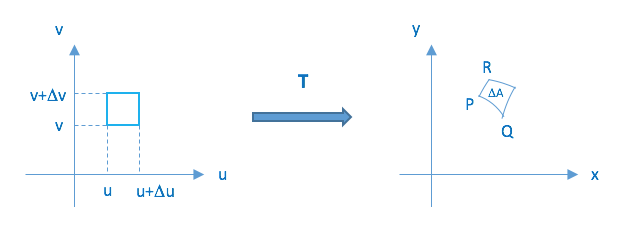
\includegraphics[width=0.7\textwidth]{change_figure}}
\caption{Figure 1: The transformation $T$ : $\(\mathbb{R}\)^2$ \rightarrow $\(\mathbb{R}\)^2$}
\end{figure}

By definition, we have
\begin{gather*} 
P = T(u,v) = (x(x,v),y(u,v)) \\
Q = T(u+\Delta u,v) = (x(u+\Delta u,v),y(u+\Delta u,v) \\
R = T(u,v+\Delta v) = (x(u,v+\Delta v),y(u,v+\Delta v)
\end{gather*}

\end{thm}


\begin{thebibliography}{1}
\bibitem{stewart12}{\sc J. Stewart}, {\em Calculus, Early Transcendentals}, Cengage Learning, 2012.
\end{thebibliography}

\end{document}